\documentclass{../../PublicResources/DocClass}

    \DocumentTitle{「软件」学习笔记}
    \DocumentCreatedDate{2020/12/18}

    \LinkBlogPost{}
    \LinkPDFSource{}
    \LinkVideo{}

    \AuthorName{Mr. Kin}
    \AuthorEmail{im.misterkin@gmail.com}
    \AuthorBlog{https://mister-kin.github.io/}

\begin{document}
    \pagenumbering{Roman} % 大写罗马字母样式页码。
    \maketitle
    \addcontentsline{toc}{chapter}{封面}
    \frontmatter
    \phantomsection
\begin{center}
    {\bfseries\sffamily\Large 关于作者}
\end{center}
\addcontentsline{toc}{chapter}{关于作者}

\subsection*{\bfseries \sffamily 关于我}
\begin{wrapfigure}[3]{L}{60pt}
    \vspace*{-20pt}
    \centering
    
\includegraphics{kin-logo}
\end{wrapfigure}
\textbf{Mr. Kin},广东客家仁,程序猿,CG和游戏爱好者,一枚极客。翻译UP主,个人UP主。不定时在B站直播日常:码代码,码博客,翻译,做视频,做教程。 ($\vartheta$$\bullet$\_$\bullet$)$\vartheta$ \hyperlink{follow}{\emph{(点击关注我!)}}

\subsection*{\bfseries \sffamily 开源建设}

\noindent {\bfseries \sffamily 开源软件的中文化翻译}

\begin{itemize}
    \item \href{https://docs.krita.org/zh_CN/}{Krita手册}:2018.8.5 - \href{https://crowdin.com/profile}{2019.4.23}
    \item \href{https://docs.blender.org/manual/zh-hans/latest/}{Blender手册}:2019.7.20 - \href{https://www.blendercn.org/5812.html?tdsourcetag=s_pctim_aiomsg}{2019.9.4} - 至今(\href{https://developer.blender.org/p/Mr_Kin/}{翻译维护})
\end{itemize}

\subsection*{\bfseries \sffamily \hypertarget{contact}{联系方式}}
\vspace*{-1ex}
\noindent {\footnotesize \color{red} \em 注:联系时请注明身份,谢谢!}

\begin{itemize}
    \item QQ:\href{tencent://AddContact/?fromId=45&fromSubId=1&subcmd=all&uin=2312463626&website=www.oicqzone.com}{2312463626}\emph{\color{red}(点击号码加好友)}
    \item 邮箱:2312463626@qq.com ; im.misterkin@gmail.com
\end{itemize}

\subsection*{\bfseries \sffamily \hypertarget{follow}{关注渠道}}
\vspace*{-1ex}
\noindent {\footnotesize \color{red} \em 注:点击文字即可跳转关注!}
\vspace*{-2ex}

\begin{figure}[htbp]
    \centering
    
\includegraphics[scale=0.2]{WechatOfficialAccounts.png}
\end{figure}
\vspace*{-4ex}

\begin{figure}[htbp]
    \centering
    \begin{minipage}[t]{0.2\textwidth}
        \centering
        \caption*{\href{https://mister-kin.github.io}{博客 - Blog}}
        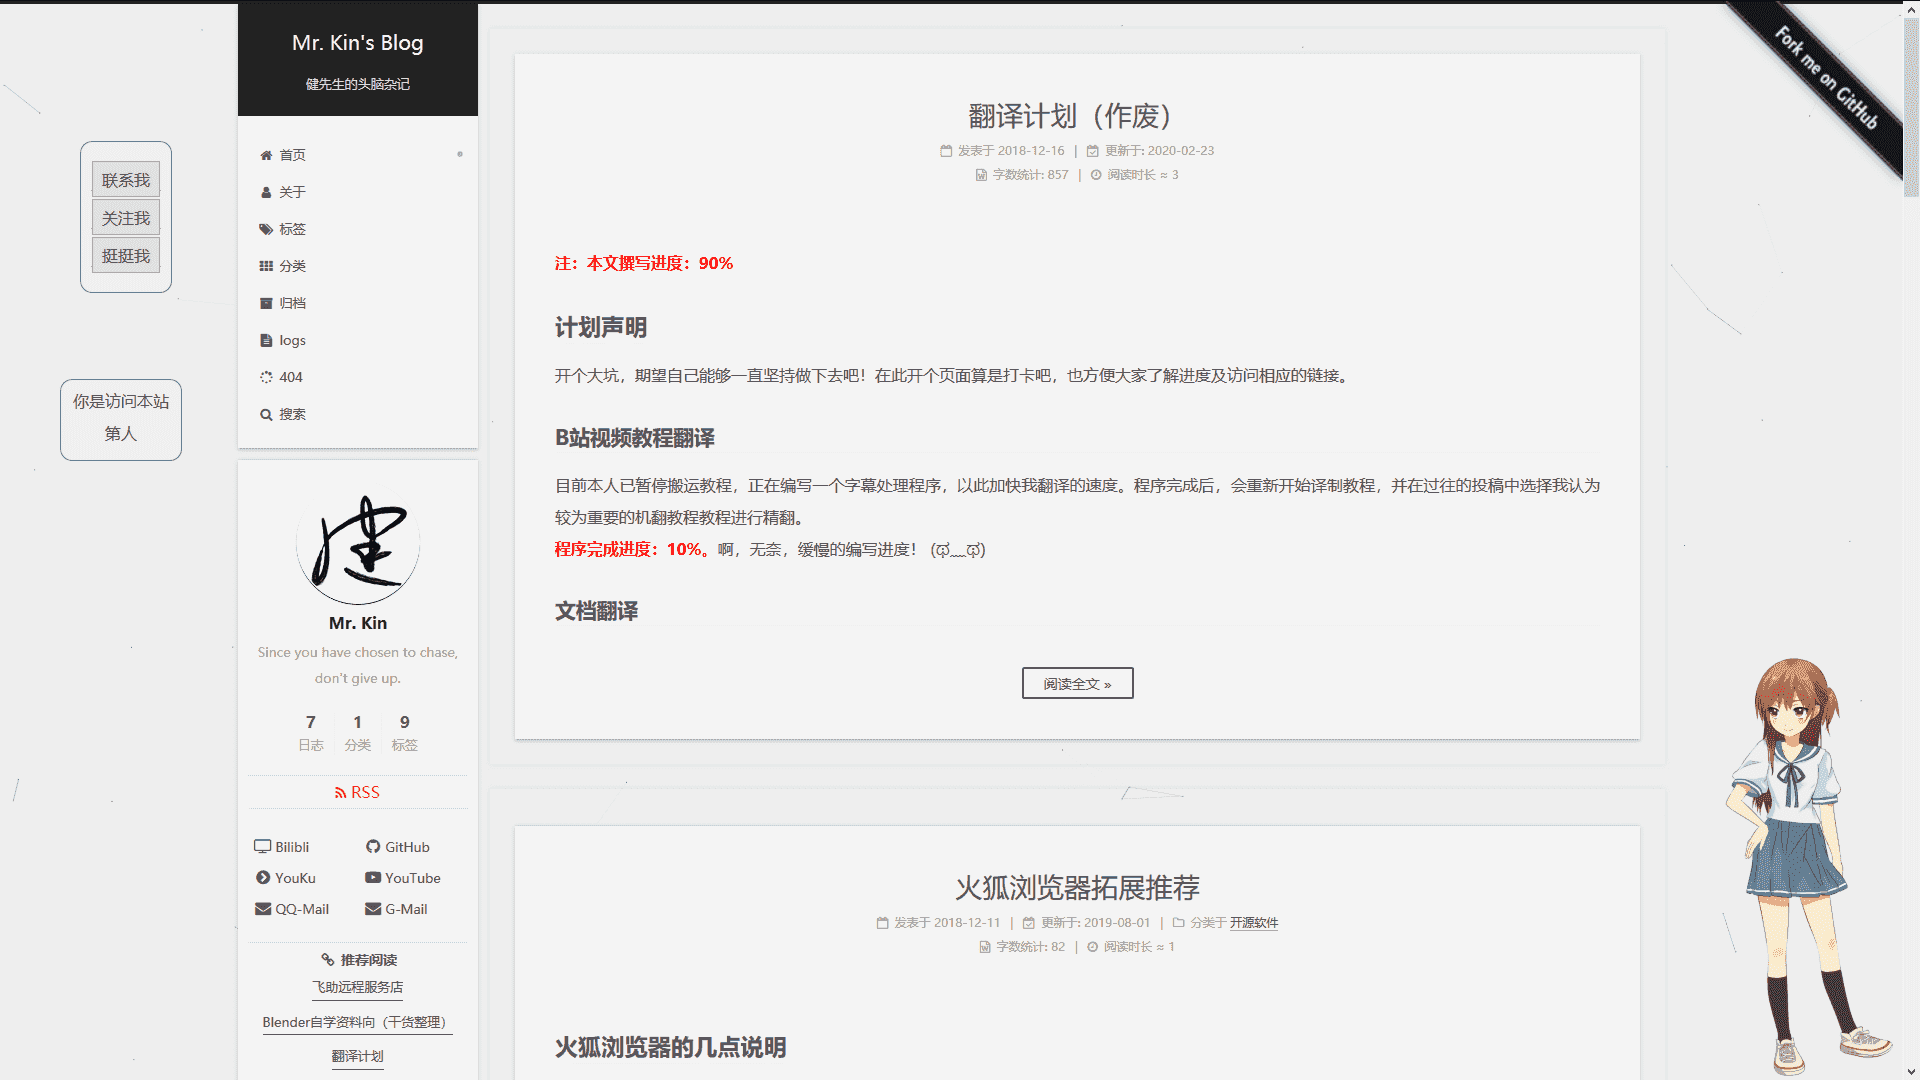
\includegraphics[scale=0.055]{Blog}
    \end{minipage}
    \qquad
    \begin{minipage}[t]{0.2\textwidth}
        \centering
        \caption*{\href{https://github.com/mister-kin}{Github}}
        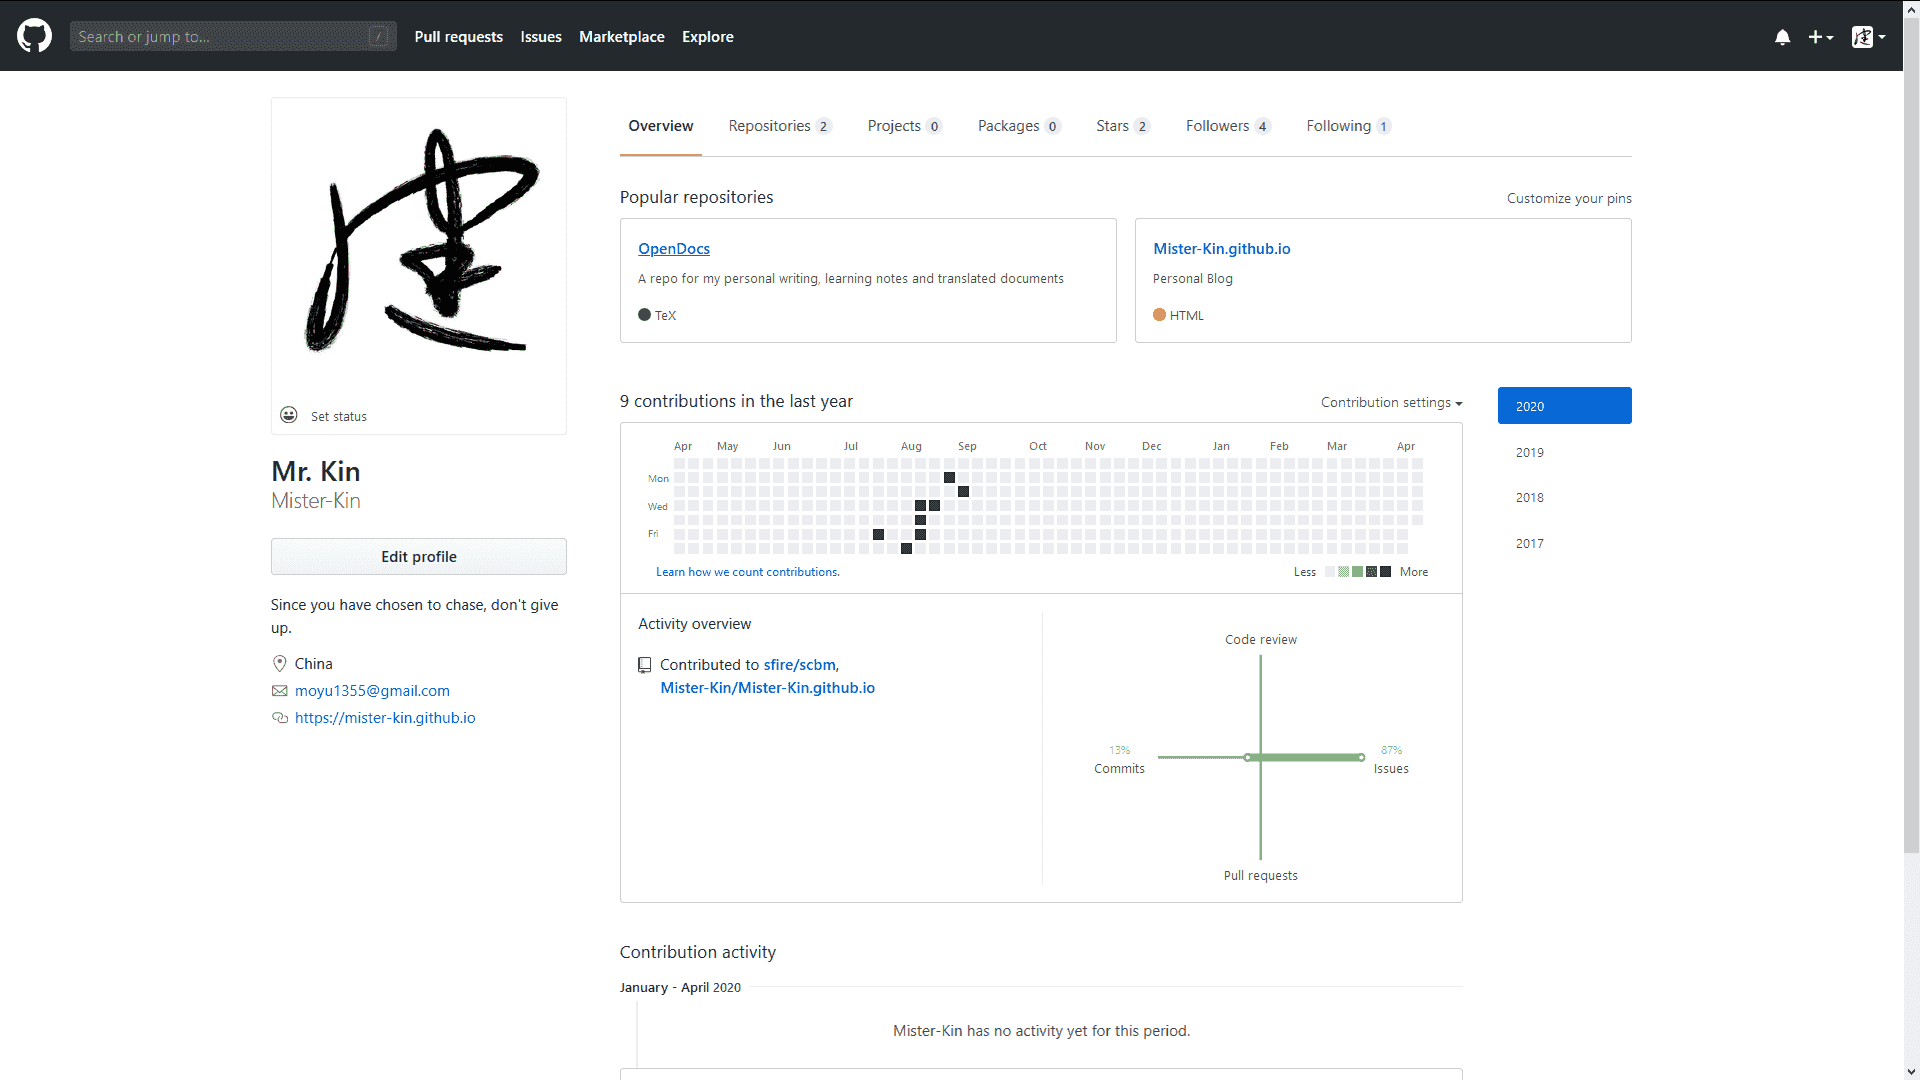
\includegraphics[scale=0.055]{Github}
    \end{minipage}
    \qquad
    \begin{minipage}[t]{0.2\textwidth}
        \centering
        \caption*{\href{https://weibo.com/6270111192/profile?topnav=1&wvr=6&is_all=1}{微博 - Weibo}}
        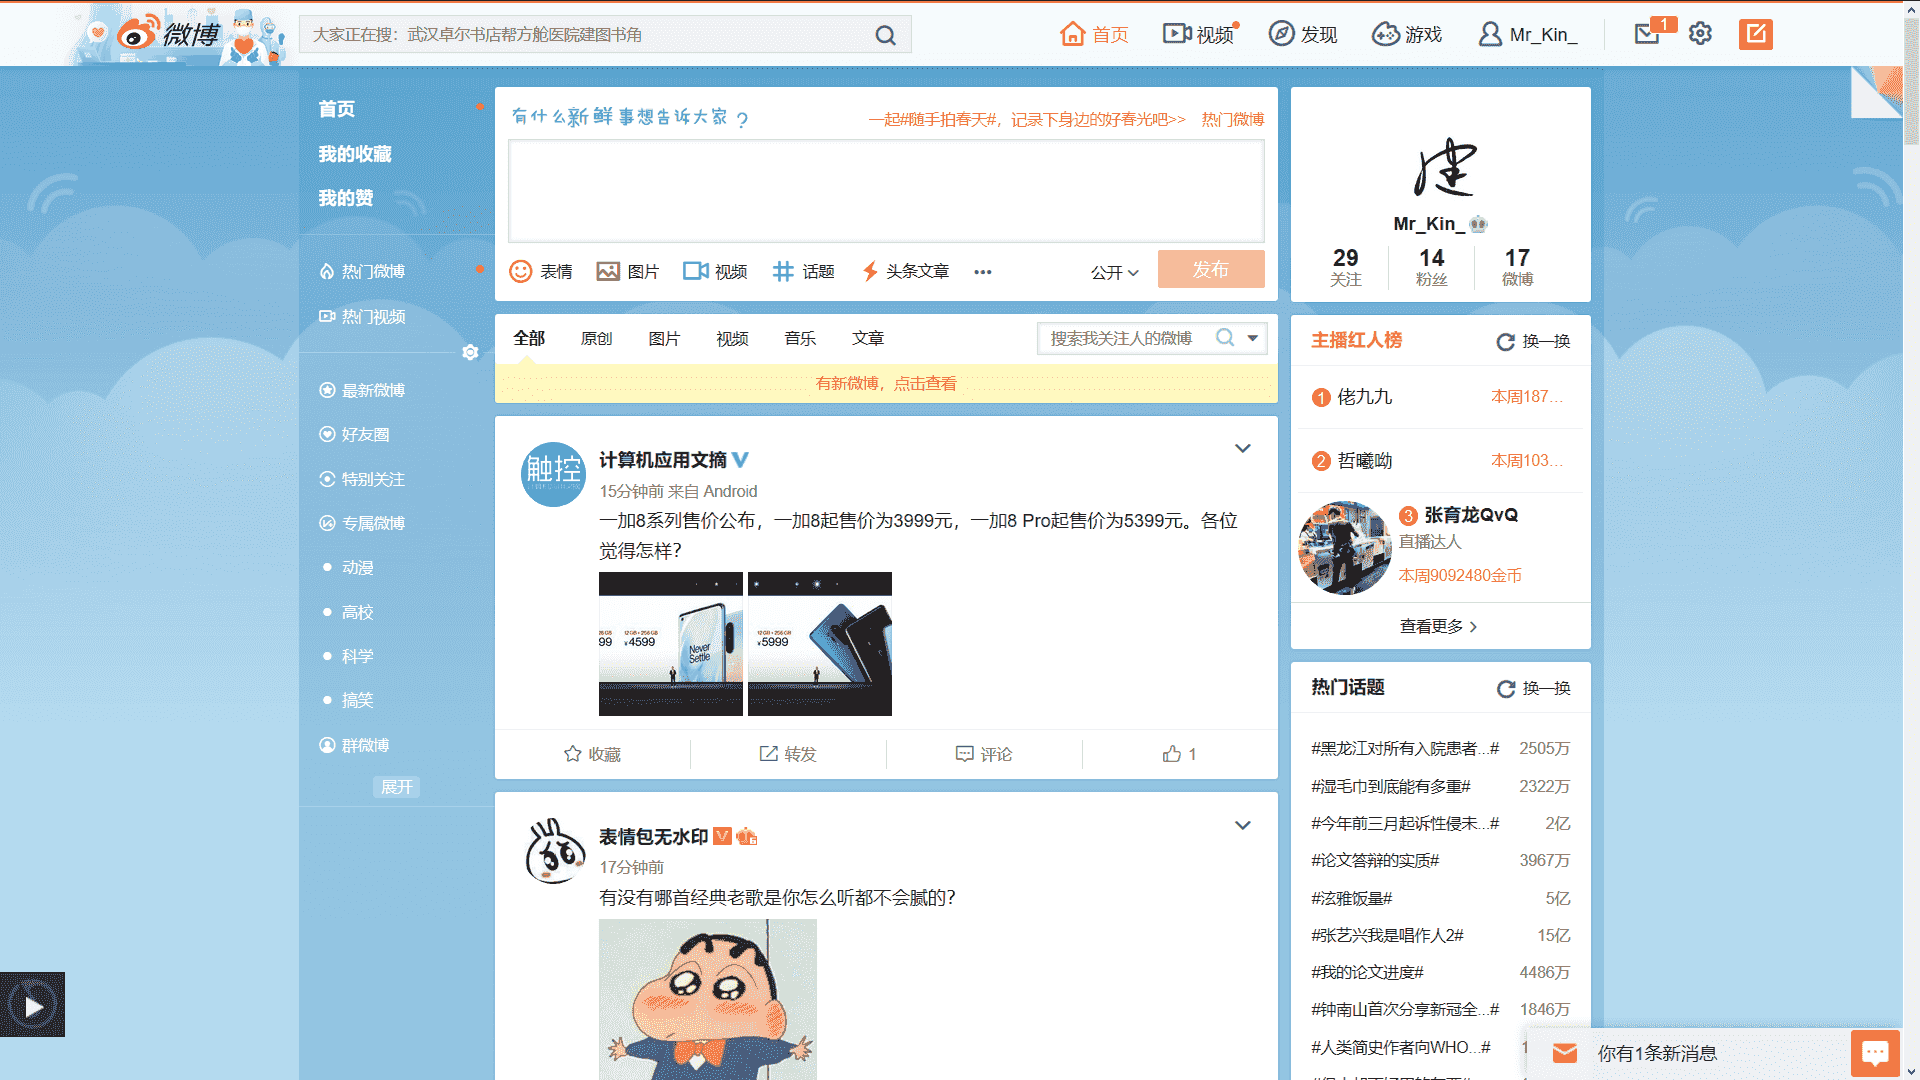
\includegraphics[scale=0.055]{Weibo}
    \end{minipage}
    \qquad
    \begin{minipage}[t]{0.2\textwidth}
        \centering
        \caption*{\href{https://www.zhihu.com/people/drwu-94}{知乎 - Zhihu}}
        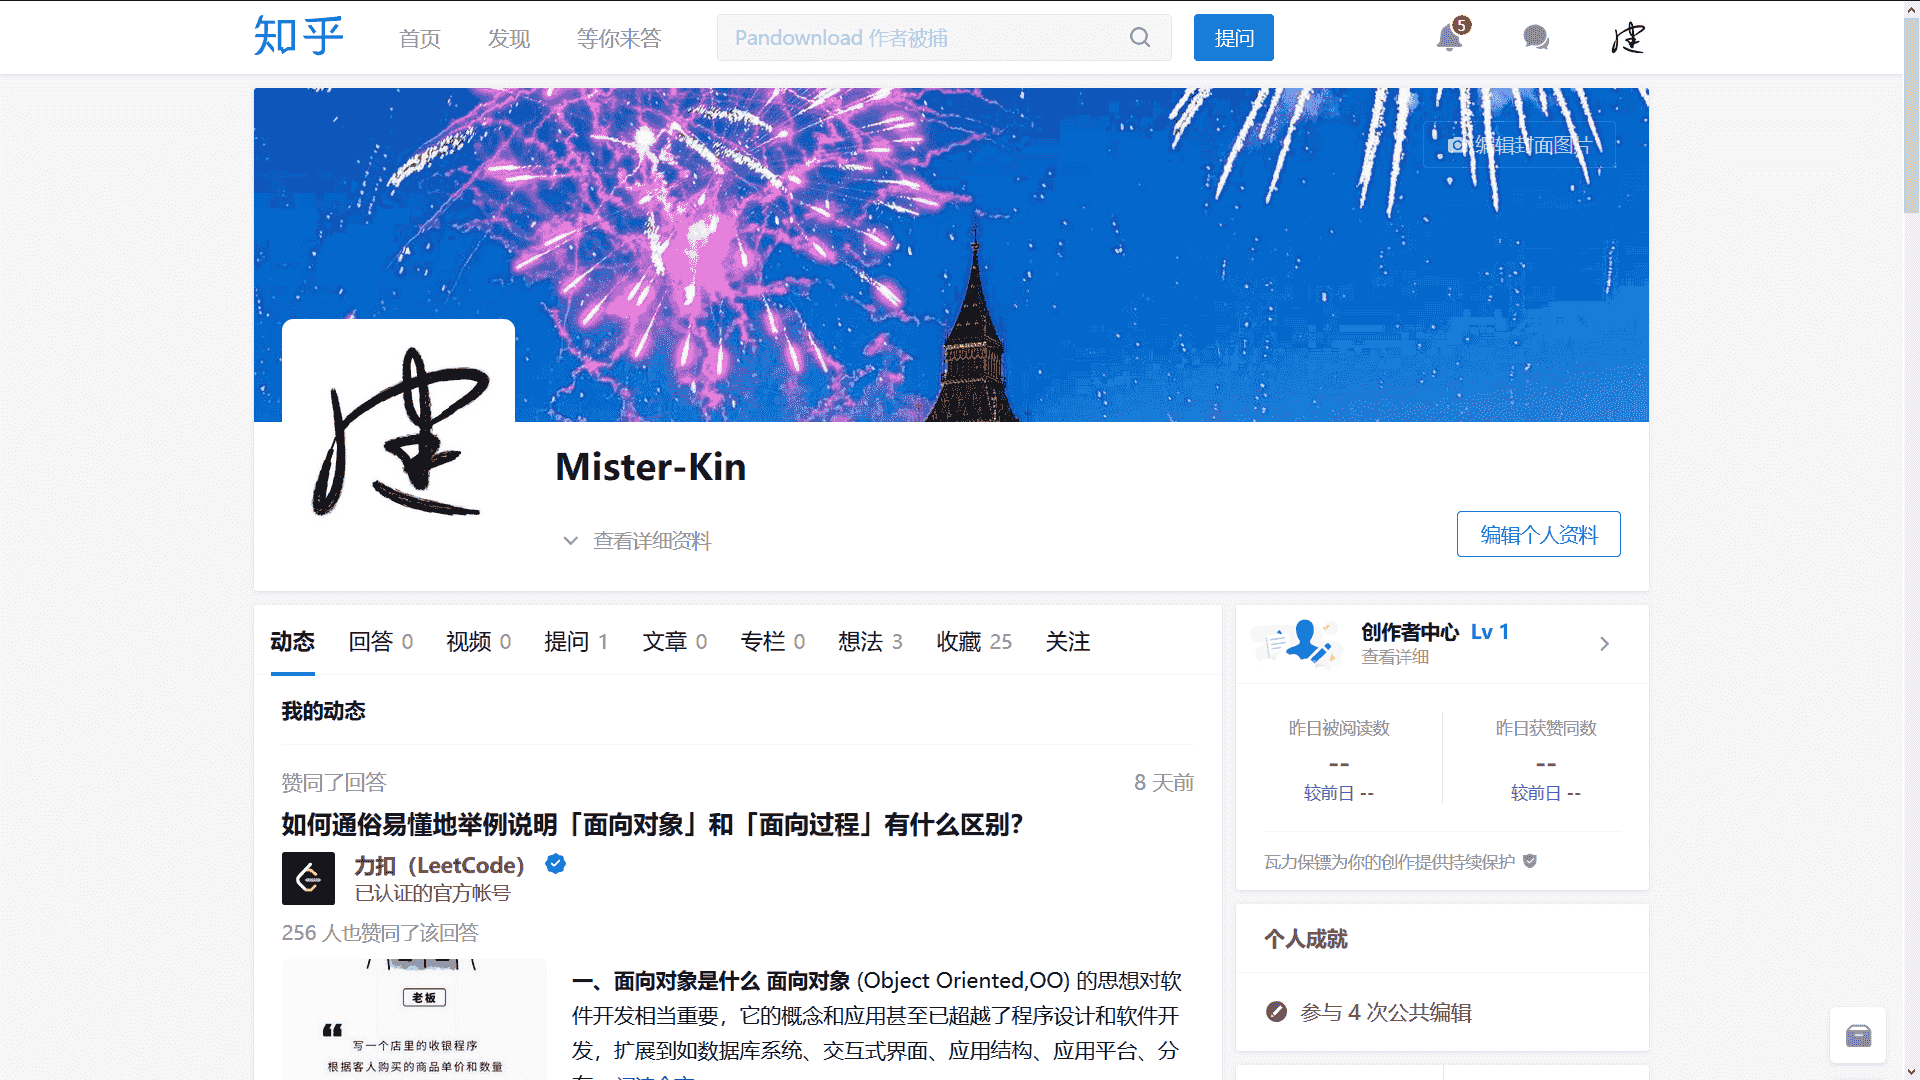
\includegraphics[scale=0.055]{Zhihu}
    \end{minipage}

    \vspace*{3ex}

    \begin{minipage}[t]{0.2\textwidth}
        \centering
        \caption*{\href{http://space.bilibili.com/17025250?}{B站 - Bilibili}}
        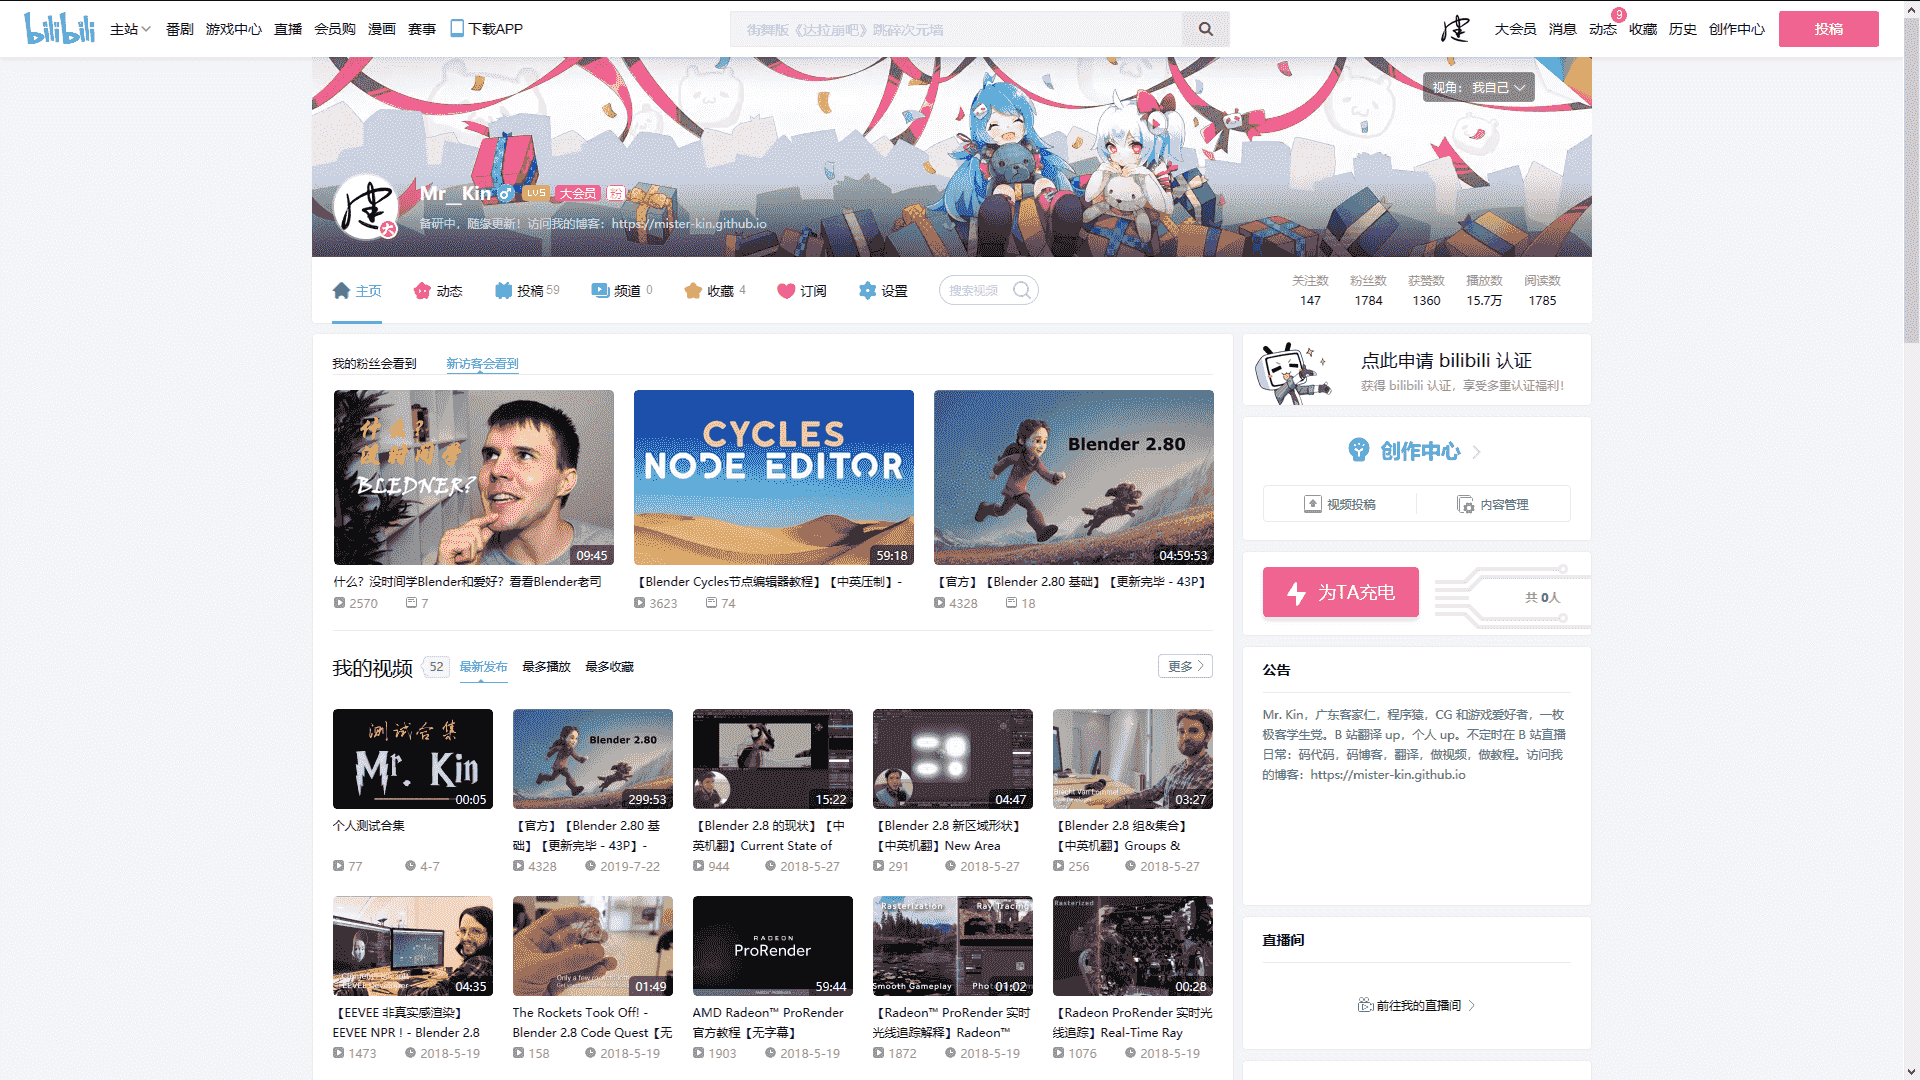
\includegraphics[scale=0.055]{Bilibili}
    \end{minipage}
    \qquad
    \begin{minipage}[t]{0.2\textwidth}
        \centering
        \caption*{\href{http://i.youku.com/i/UNjA3MTk5Mjgw?spm=a2hzp.8253869.0.0}{优酷 - Youku}}
        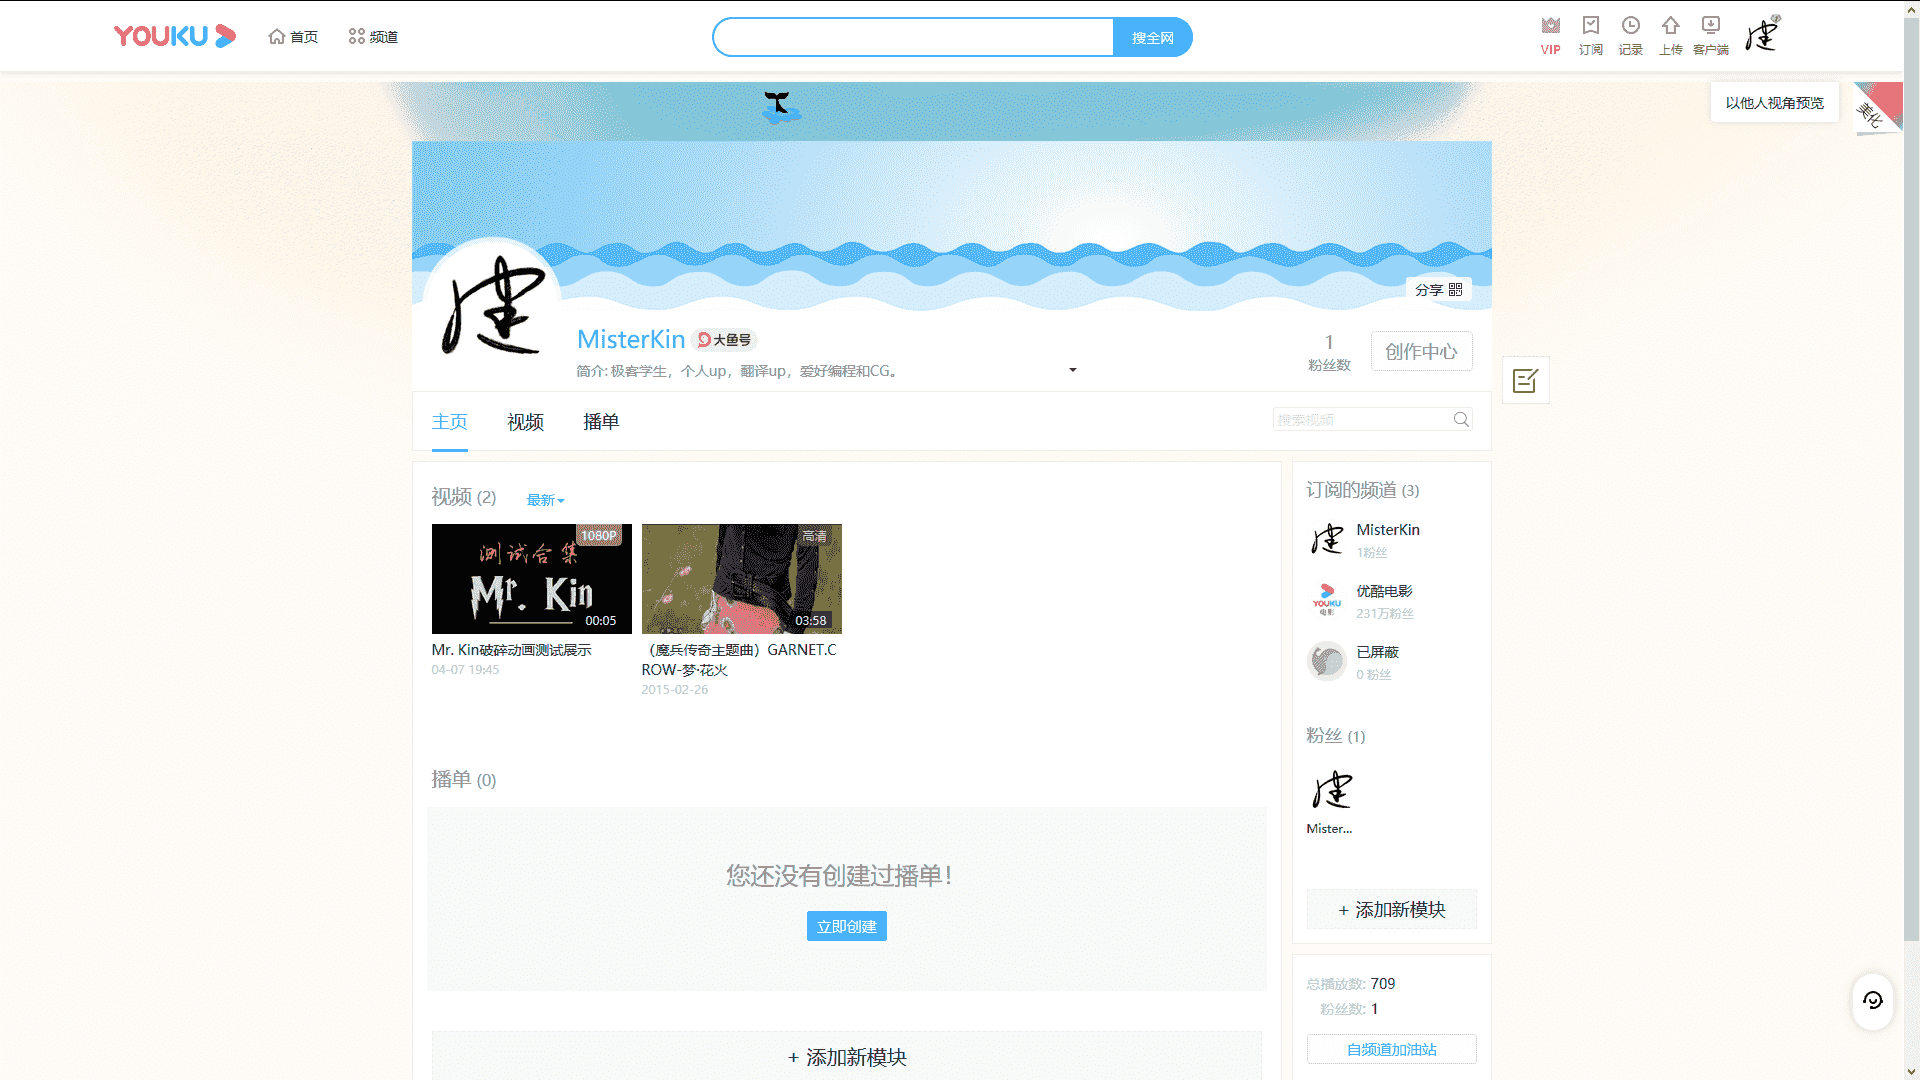
\includegraphics[scale=0.055]{Youku}
    \end{minipage}
    \qquad
    \begin{minipage}[t]{0.2\textwidth}
        \centering
        \caption*{\href{https://www.toutiao.com/c/user/835254071079053/\#mid=1663279303982091}{头条 - Headline}}
        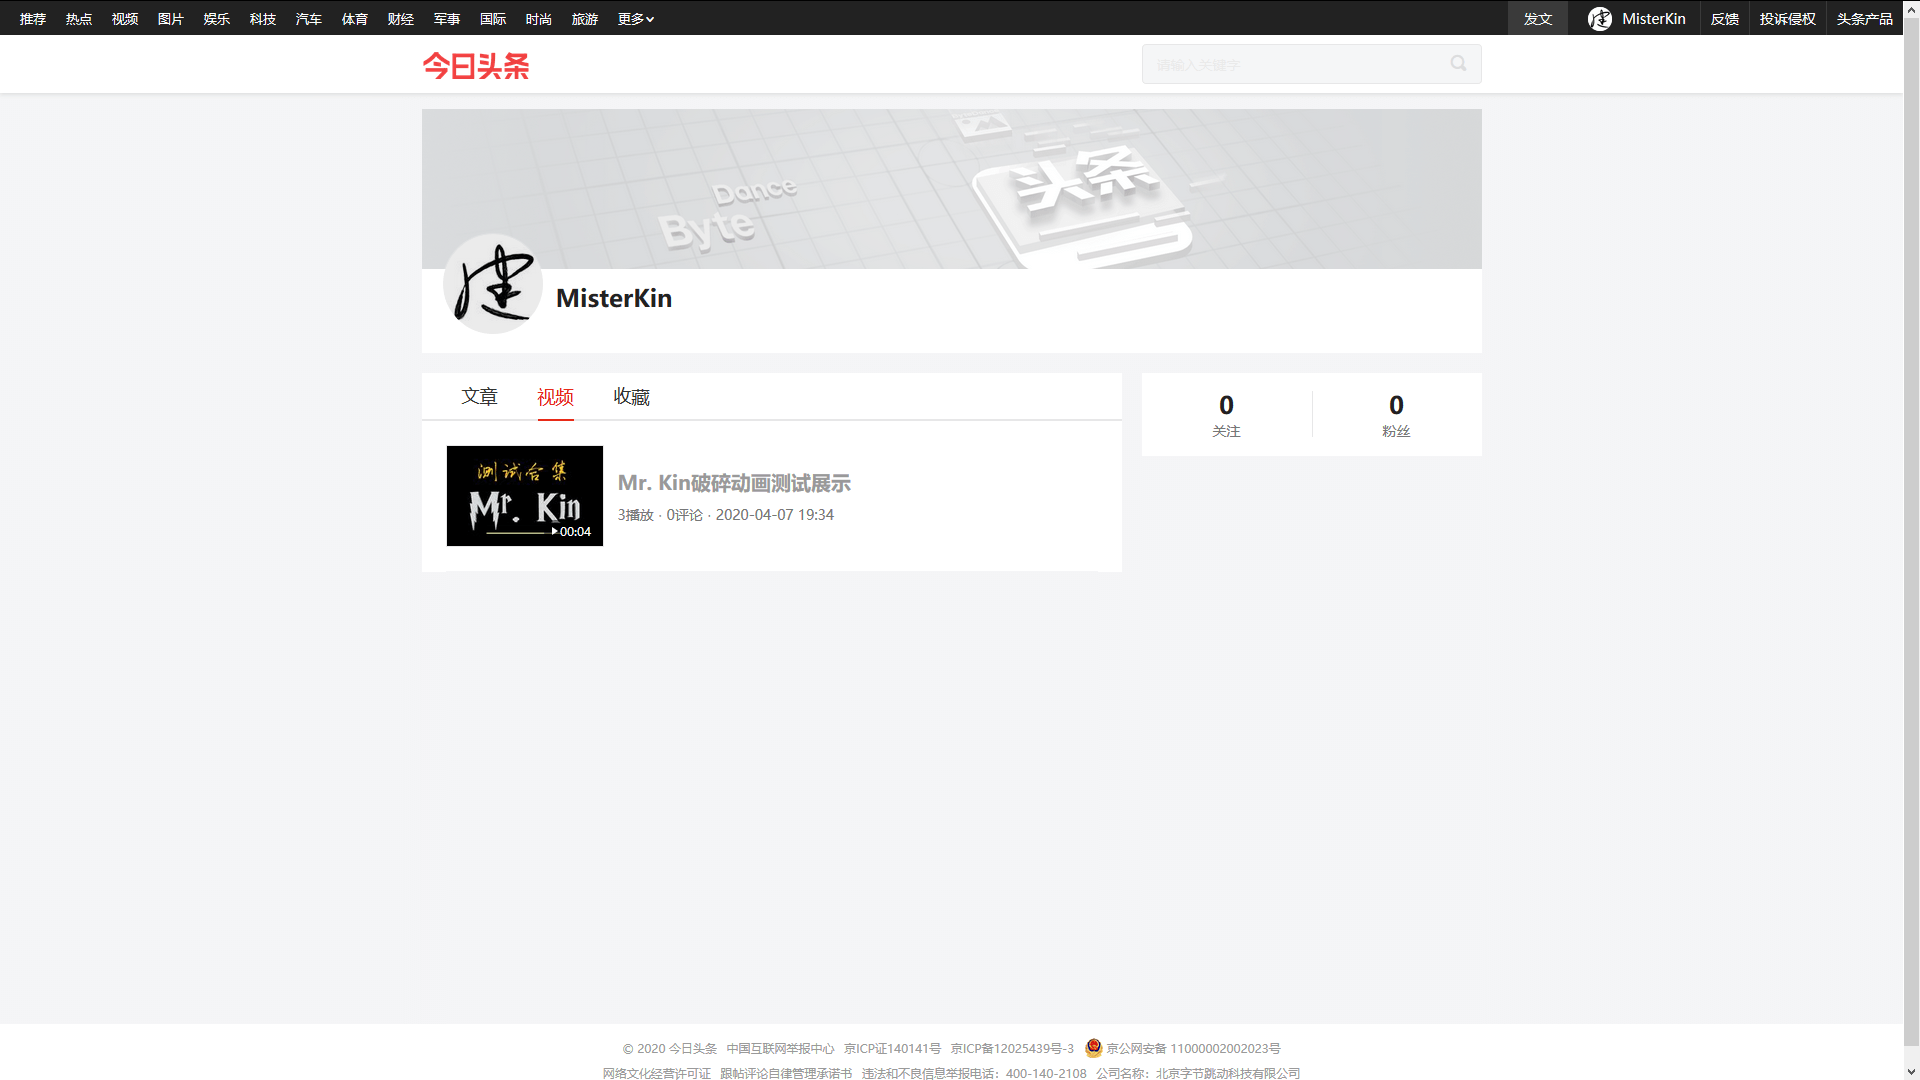
\includegraphics[scale=0.055]{Headline}
    \end{minipage}
    \qquad
    \begin{minipage}[t]{0.2\textwidth}
        \centering
        \caption*{\href{https://www.youtube.com/channel/UCXqjfWLzMlRKxGC8syWj17Q?view_as=public}{油管 - Youtube}}
        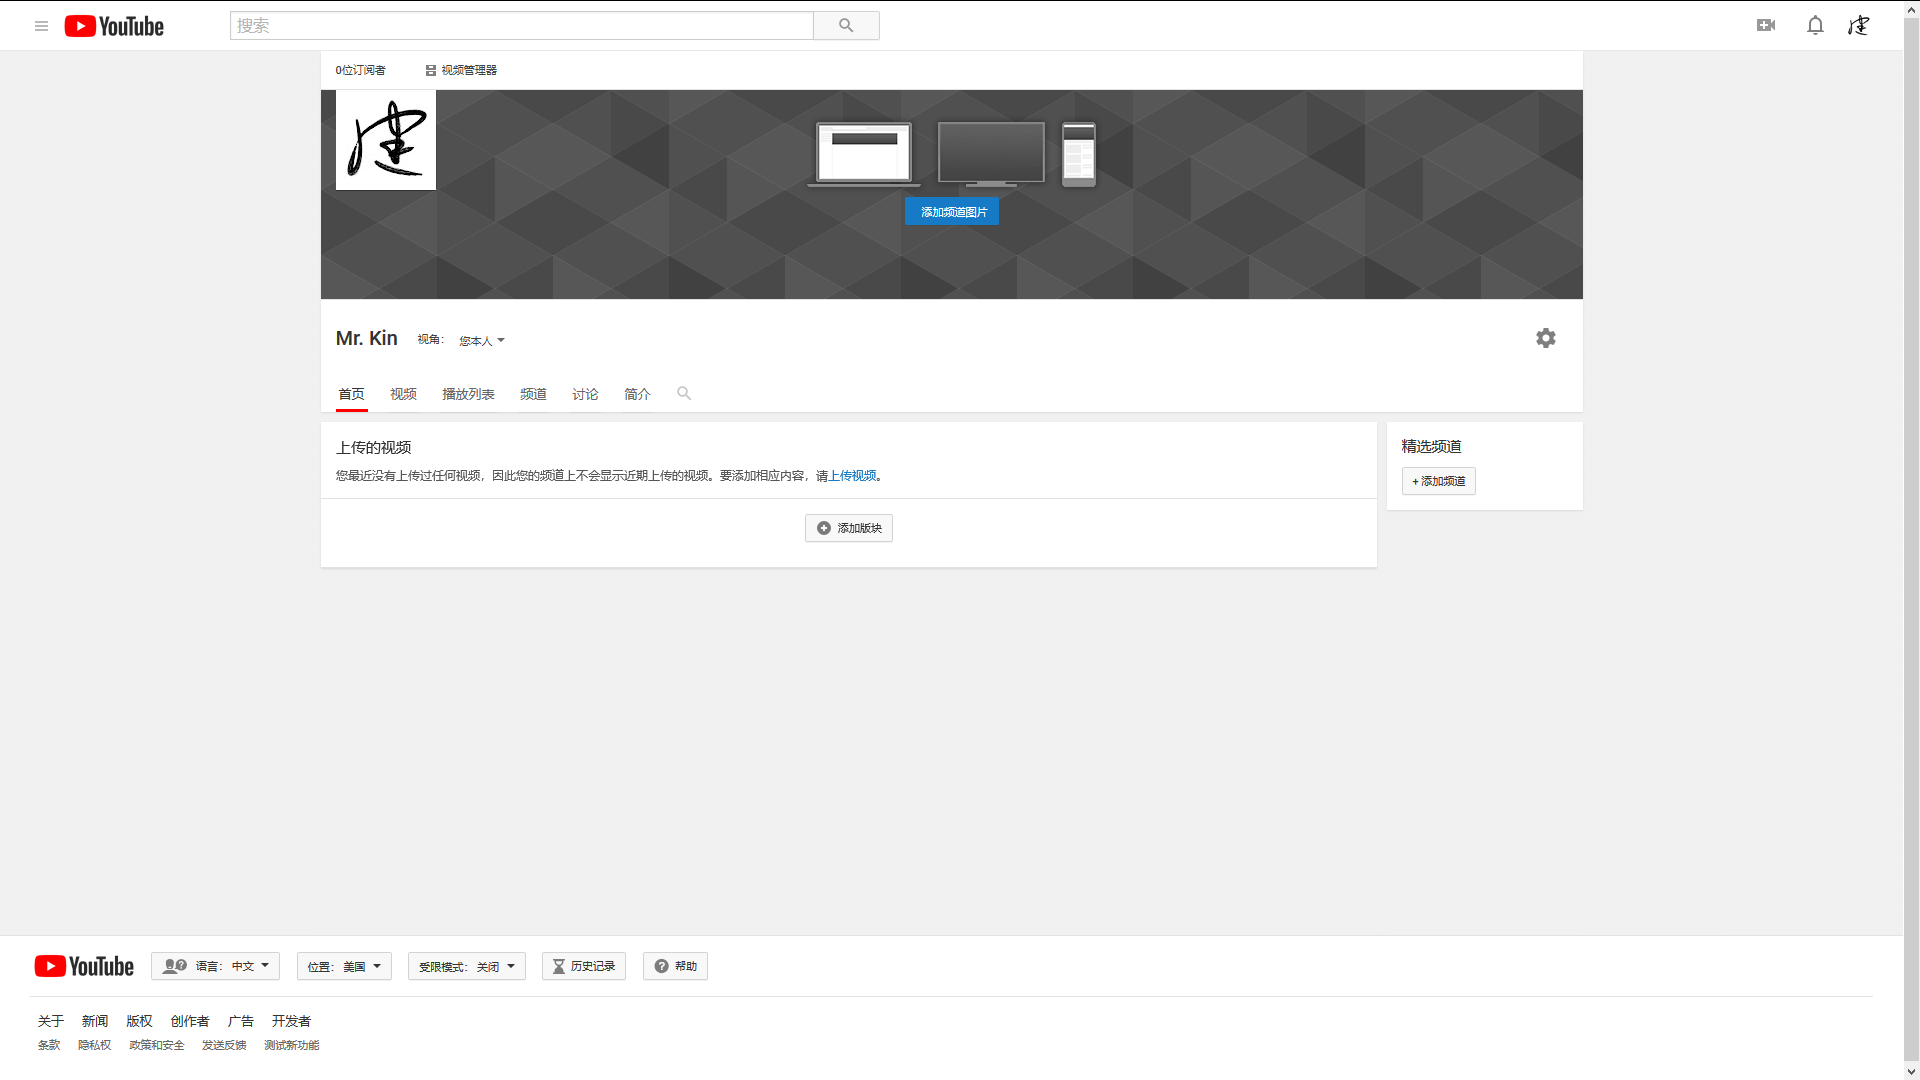
\includegraphics[scale=0.055]{Youtube}
    \end{minipage}
\end{figure}
 % 出于特殊的安全设置,\include 命令无法使用相对路径,因为需要读写权限以给 included file 写 aux 文件,而 \input 命令只需要读权限。
    \clearpage
    \phantomsection
\begin{center}
    {\bfseries\sffamily\Large 版权声明}
\end{center}
\addcontentsline{toc}{chapter}{版权声明}

\noindent 作者:Mr. Kin \\
\DetectToksEmpty\LinkBlogPost
\ifToksEmpty
博文链接:链接暂空\\
\else
博文链接:\href{\the\LinkBlogPost}{跳转博文页}\\
\fi
\DetectToksEmpty\LinkPDFSource
\ifToksEmpty
PDF及LaTex源码链接:链接暂空\\
\else
PDF及LaTex源码链接:\href{\the\LinkPDFSource}{跳转PDF及LaTex源码页}\\
\fi
\DetectToksEmpty\LinkVideo
\ifToksEmpty
\else
相关视频创作链接:\href{\the\LinkVideo}{跳转视频页}\\
\fi
许可协议:本作品的所有内容,除个人设计创作的图像(如logo等)和相关的视频创作及其他特别声明外,均采用\href{https://creativecommons.org/licenses/by-nc-sa/4.0/deed.zh}{知识共享\ 署名-非商业性使用-相同方式共享 4.0 国际许可协议}进行发布。版权 © Mr. Kin,保留所有权利。
\includegraphics[scale=.4]{CC-BY-NC-SA}\\*[1.3ex]
\begin{tabular}{|*{3}{p{0.306\textwidth}|}}
    \hline
    \textsf{\bfseries 允许} & \textsf{\bfseries 限制} & \textsf{\bfseries 条件} \\
    \hline
    \vspace{-8pt}{\color{green}√} 修改 & \vspace{-8pt}{\color{red}×} 商标使用 & \vspace{-8pt}{\color{blue}$\odot$} 保留原署名 \\[-12pt]
    {\color{green}√} 分发 & {\color{red}×} 专利使用 & {\color{blue}$\odot$} 状态变更说明 \\[-12pt]
    {\color{green}√} 个人使用 & {\color{red}×} 商业使用 & {\color{blue}$\odot$} 相同的许可和版权声明 \\
    \hline
\end{tabular}
\\*[1.3ex]
\emph{注:若想对本作品进行转载、引用亦或是进行二次创作时,请详细阅读上述相关协议内容(若不理解,请点击链接跳转阅读)。为保障本人权利,对于违反者,本人将依法予以处理!望周知!——Mr. Kin}

\begin{center}
    {\bfseries\sffamily\Large 勘误声明}
\end{center}

虽本人写作时已尽力保证其内容的正确性,但因个人知识面和经验的局限性以及计算机技术等相关技术日新月异,本作品内容或存在一些错误之处。还望诸君发现错误后能够\hyperlink{contact}{联系我}以更正错误,不胜感激!——Mr. Kin

\begin{center}
    {\bfseries\sffamily\Large 侵权声明}
\end{center}

若本作品采用的第三方内容侵犯了你的版权,请与我\hyperlink{contact}{联系}进行处理,谢谢!——Mr. Kin

\begin{center}
    {\bfseries\sffamily\Large 第三方开源许可声明}
\end{center}

\noindent 本作品使用的第三方开源产品有:
\begin{multicols}{2}
\begin{itemize}
    \item \href{https://github.com/adobe-fonts}{Adobe Fonts}: \href{https://github.com/adobe-fonts/source-serif-pro/blob/release/LICENSE.md}{OFL v1.1}
    \item \href{https://tug.org/texlive/}{Tex Live}: \href{https://tug.org/texlive/copying.html}{TeX Live Licensing}
    \item \href{https://code.visualstudio.com/}{Visual Studio Code}: \href{https://github.com/Microsoft/vscode/blob/master/LICENSE.txt}{MIT}
    \item \href{http://ffmpeg.org/}{FFmpeg}: \href{http://ffmpeg.org/legal.html}{LGPL v2.1 / GPL v2}
    \item \href{https://krita.org/en/}{Krita}: \href{https://docs.krita.org/en/KritaFAQ.html?highlight=license#license-rights-and-the-krita-foundation}{Krita's GPL license}
    \item \href{https://inkscape.org/}{Inkscape}: \href{https://inkscape.org/about/license/}{GPL}
    \item \href{https://www.gimp.org}{GIMP}: \href{https://www.gimp.org/about/COPYING}{GPL}
    \item \href{https://www.blender.org}{Blender}: \href{https://www.blender.org/about/license/}{GPL}
    \item \href{https://www.audacityteam.org/}{Audacity}: \href{https://www.audacityteam.org/about/license/}{GPL v2}
    \item \href{https://handbrake.fr}{Handbrake}: \href{https://github.com/HandBrake/HandBrake/blob/master/LICENSE}{GPL v2}
\end{itemize}
\end{multicols}

\noindent 更多请点击查看\href{https://mister-kin.github.io/about/third-party-declaration/}{第三方声明页}!

    \clearpage
    {\centering \tableofcontents} % 生成目录页。
    \mainmatter

    % 正文
    \input{Shortcuts/Shortcuts}
    % Blender
\chapter{Blender}
\section{3D视窗}

\begin{intro}
    3D视图用于与3D场景交互以用于各种目的,例如建模、动画、纹理绘制等。
\end{intro}

\subsection{选择-菜单>选择}
\begin{itemize}
    \item 选择物体:「左键」物体
    \item 取消选择:「左键」空白处
    \item 全选:「A」
    \item 取消全选:「Alt+A」
\end{itemize}

\subsection{视窗导航-菜单>视图}
\begin{itemize}
    \item 旋转:「中键」或「Gizmo球体」或「数字键4862」
    \item 平移:「shift+中键」或「Gizmo手掌」
    \item 缩放:「滑轮」或「Gizmo放大镜」或「数字键-+」
    \item 查看选中对象:「数字键.」
    \item 摄像机视图:「数字键0」或「Gizmo摄像机」
\end{itemize}

\section{实战篇}

\subsection{SVG转3D网格}
\begin{enumerate}
    \item 切换到顶视图-7键。
    \item 菜单>文件>导入>SVG
    \item 缩放视图找到SVG。
    \item 右键set origin,调整“原点”至物体中心。
    \item shift+s键对齐“原点”至世界中心
    \item 选中并缩放至合适大小。
    \item 右键convert to,转换到Mesh。
    \item 选中网格物体,TAB键进入“编辑模式”。
    \item A键选中所有网格。
    \item 切换到侧视图-3或1键。(按住Ctrl时为视图反方向)
    \item E键挤出面。
    \item TAB键回到“物体模式”。
\end{enumerate}

\subsection{灰尘粒子动画}
无特殊说明,则都是在粒子标签内操作。
\begin{enumerate}
    \item 创建合适的立方体(粒子场)
    \item 选择立方体,属性编辑器>粒子标签>新建粒子系统
    \item 粒子类型>发射体;发射>源>发射源>体积
    \item 创建灰尘物体模型
    \item 渲染>渲染为>物体(此为单个效果,用集合来实现多个),物体>选择灰尘物体模型
    \item 渲染>缩放>数值调整;缩放随机性>1
    \item 1键切换到前视图,ctrl+alt+0并左击相机视角边框处以选中相机,按G调整相机视角;属性编辑器>相机属性>镜头>焦距>数值调整。
    \item 启用旋转功能>坐标系轴向>normal;随机>数值调整;相位>数值调整;随机相位>数值调整
    \item 选中立方体,属性编辑器>材质>表面>移除材质,材质>体积>原理化体积>密度调0.14
    \item 属性编辑器>世界属性>颜色调至黑色(除去环境亮度)
    \item
\end{enumerate}

\section{二次开发-插件}

\subsection{开发技巧}
用户偏好设置-开发额外选项+Python工具提示+工具提示

开启「开发额外选项」后,右键UI组件,可以查看源代码。

在寻找UI组件所在类目时,可查看Python工具提示信息。

在查找一些操作命令时,可以在blender里操作后在控制台看执行的语句。活用blender控制台进行调试。

\subsection{常见API总结}
\begin{itemize}
    \item 插件信息说明:\href{https://wiki.blender.org/wiki/Process/Addons/Guidelines/metainfo#Script_Meta_Info}{见info字典元素}
    \item bpy.types:Header, Menu, Panel, Operator。前三个都是需要定义draw函数来实现UI,Operator一般用来定义操作的execute函数。
\end{itemize}


% Krita
\chapter{Krita}
\section{实战篇}

\subsection{SVG转3D网格}
\begin{enumerate}
    \item 切换到顶视图-7键。
    \item 菜单>文件>导入>SVG
    \item 缩放视图找到SVG。
    \item 右键set origin,调整“原点”至物体中心。
    \item shift+s键对齐“原点”至世界中心
    \item 选中并缩放至合适大小。
    \item 右键convert to,转换到Mesh。
    \item 选中网格物体,TAB键进入“编辑模式”。
    \item A键选中所有网格。
    \item 切换到侧视图-3或1键。(按住Ctrl时为视图反方向)
    \item E键挤出面。
    \item TAB键回到“物体模式”。
\end{enumerate}

\subsection{灰尘粒子动画}
无特殊说明,则都是在粒子标签内操作。
\begin{enumerate}
    \item 创建合适的立方体(粒子场)
    \item 选择立方体,属性编辑器>粒子标签>新建粒子系统
    \item 粒子类型>发射体;发射>源>发射源>体积
    \item 创建灰尘物体模型
    \item 渲染>渲染为>物体(此为单个效果,用集合来实现多个),物体>选择灰尘物体模型
    \item 渲染>缩放>数值调整;缩放随机性>1
    \item 1键切换到前视图,ctrl+alt+0并左击相机视角边框处以选中相机,按G调整相机视角;属性编辑器>相机属性>镜头>焦距>数值调整。
    \item 启用旋转功能>坐标系轴向>normal;随机>数值调整;相位>数值调整;随机相位>数值调整
    \item 选中立方体,属性编辑器>材质>表面>移除材质,材质>体积>原理化体积>密度调0.14
    \item 属性编辑器>世界属性>颜色调至黑色(除去环境亮度)
    \item
\end{enumerate}


% Inkscape
\chapter{Inkscape}
\section{实战篇}

\subsection{SVG转3D网格}
\begin{enumerate}
    \item 切换到顶视图-7键。
    \item 菜单>文件>导入>SVG
    \item 缩放视图找到SVG。
    \item 右键set origin,调整“原点”至物体中心。
    \item shift+s键对齐“原点”至世界中心
    \item 选中并缩放至合适大小。
    \item 右键convert to,转换到Mesh。
    \item 选中网格物体,TAB键进入“编辑模式”。
    \item A键选中所有网格。
    \item 切换到侧视图-3或1键。(按住Ctrl时为视图反方向)
    \item E键挤出面。
    \item TAB键回到“物体模式”。
\end{enumerate}

\subsection{灰尘粒子动画}
无特殊说明,则都是在粒子标签内操作。
\begin{enumerate}
    \item 创建合适的立方体(粒子场)
    \item 选择立方体,属性编辑器>粒子标签>新建粒子系统
    \item 粒子类型>发射体;发射>源>发射源>体积
    \item 创建灰尘物体模型
    \item 渲染>渲染为>物体(此为单个效果,用集合来实现多个),物体>选择灰尘物体模型
    \item 渲染>缩放>数值调整;缩放随机性>1
    \item 1键切换到前视图,ctrl+alt+0并左击相机视角边框处以选中相机,按G调整相机视角;属性编辑器>相机属性>镜头>焦距>数值调整。
    \item 启用旋转功能>坐标系轴向>normal;随机>数值调整;相位>数值调整;随机相位>数值调整
    \item 选中立方体,属性编辑器>材质>表面>移除材质,材质>体积>原理化体积>密度调0.14
    \item 属性编辑器>世界属性>颜色调至黑色(除去环境亮度)
    \item
\end{enumerate}


    % Office
\chapter{Office}
\section{Word}

\subsection{页码排版问题}
分页符前后的页眉页脚是一样的,分节符前后才有可能不一样。

分节符后面的页眉页脚一般都是默认继承前面的格式的,可以取消“链接到前一个”。

分节符用的下一页。

关于分页符和分节符的删除。
\begin{enumerate}
    \item 视图删除法:进入菜单「视图」>「大纲视图」或者「草稿视图」等,找到想要删除的符号,按delete键进行删除。
    \item 在菜单「开始」的文字样式左边,显示/隐藏编辑标记(箭头符号)。点击显示符号,然后delete删除。
\end{enumerate}

\subsection{格式刷}
选中需要复制样式的文字,然后点击菜单「开始」>「格式刷」。然后选中其他需要应用的文字。

单击时,只能使用一次。双击时,能多次使用。

\subsection{自动目录}
在菜单「视图」>「大纲视图」对需要生成目录的标题进行级别排版后,点击菜单「引用」>「目录」>「自动目录1」。



    \nocite{*} % 不使用 cite 也能生成参考文献。
    \printbibliography % 生成参考文献排版。
    \addcontentsline{toc}{chapter}{参考文献} % 添加参考文献进目录。

    \appendix
    % 附录

\end{document}
